% Descrivere cosa c'è di interessante nella cattura evidenziando i MAC che conosciamo, quelli che 
% fanno cose che abbiamo capito (ad esempio i sonos oppure i dispositivi che usano zoom) e inserire
% le immagini come contorno

\subsection{Sonos capture.}
%Fabio

\subsection{Zoom captures.}
%Fabio

\subsection{Multimedia internet capture.}
In this paragraph, we analyze the results obtained with a capture performed during a lecture of
multimedia internet. \\ 
The lecture has been followed using \textit{Microsoft\ Teams}: the professor was presenting the
topic sharing its screen and all the students were following him with camera and microphone inactive.\\
In the Figure \ref{Multimedia internet lecture: data and packets exchanged.}, we can see on the
left the graphs reporting the number of bytes transmitted and received by some of the \textit{MACs}
we have revealed and on the right the number of transmitted and received by the same \textit{MACs}.\\
As we can see, there are some \textit{MACs} that are exchanging much more traffic than others:

\begin{itemize}
    \item \textbf{88:ae:07:3d:8a:30}: this is the device (an \textit{iPad\ Pro}) from which the lecture 
            was being attended. Even if the capture lasted only 5 minutes, we can see that this 
            device has received a lot of bytes (about 42.660 MB): this is of course due to the fact
            that the device was using a video-conferencing application.\\ 
            If we consider the number of packets received by this \textit{MAC}, we can compute the 
            average length of the packets during the 5 minutes of the capture:

            \begin{equation}
                \textit{Average packet length} = \textit{Number of bytes} / \textit{Number of packets} = 594 Bytes
            \end{equation}

    \item \textbf{20:b0:01:22:22:66}: this is the access point of the home were the lecture was being
            attended. Indeed, we can see that the access point has sent a lot of bytes and packets: 
            most of them were probably destined to the \textit{iPad\ Pro} that was being used to
            follow the lecture, since that device was connected to this access point while attending 
            the class. 
\end{itemize}

Among the other \textit{MAC} addresses present in the graph but that have exchanged only a few 
packets in compared with the 2 ones mentioned above, we recognize only \textbf{dc:a9:04:91:42:b9}: 
it's a \textit{MacBook Pro} in the same home. During the 5 minutes of the capture, this device was 
being used for smart-working purposes.s

\begin{figure}[h!]
    \centering
    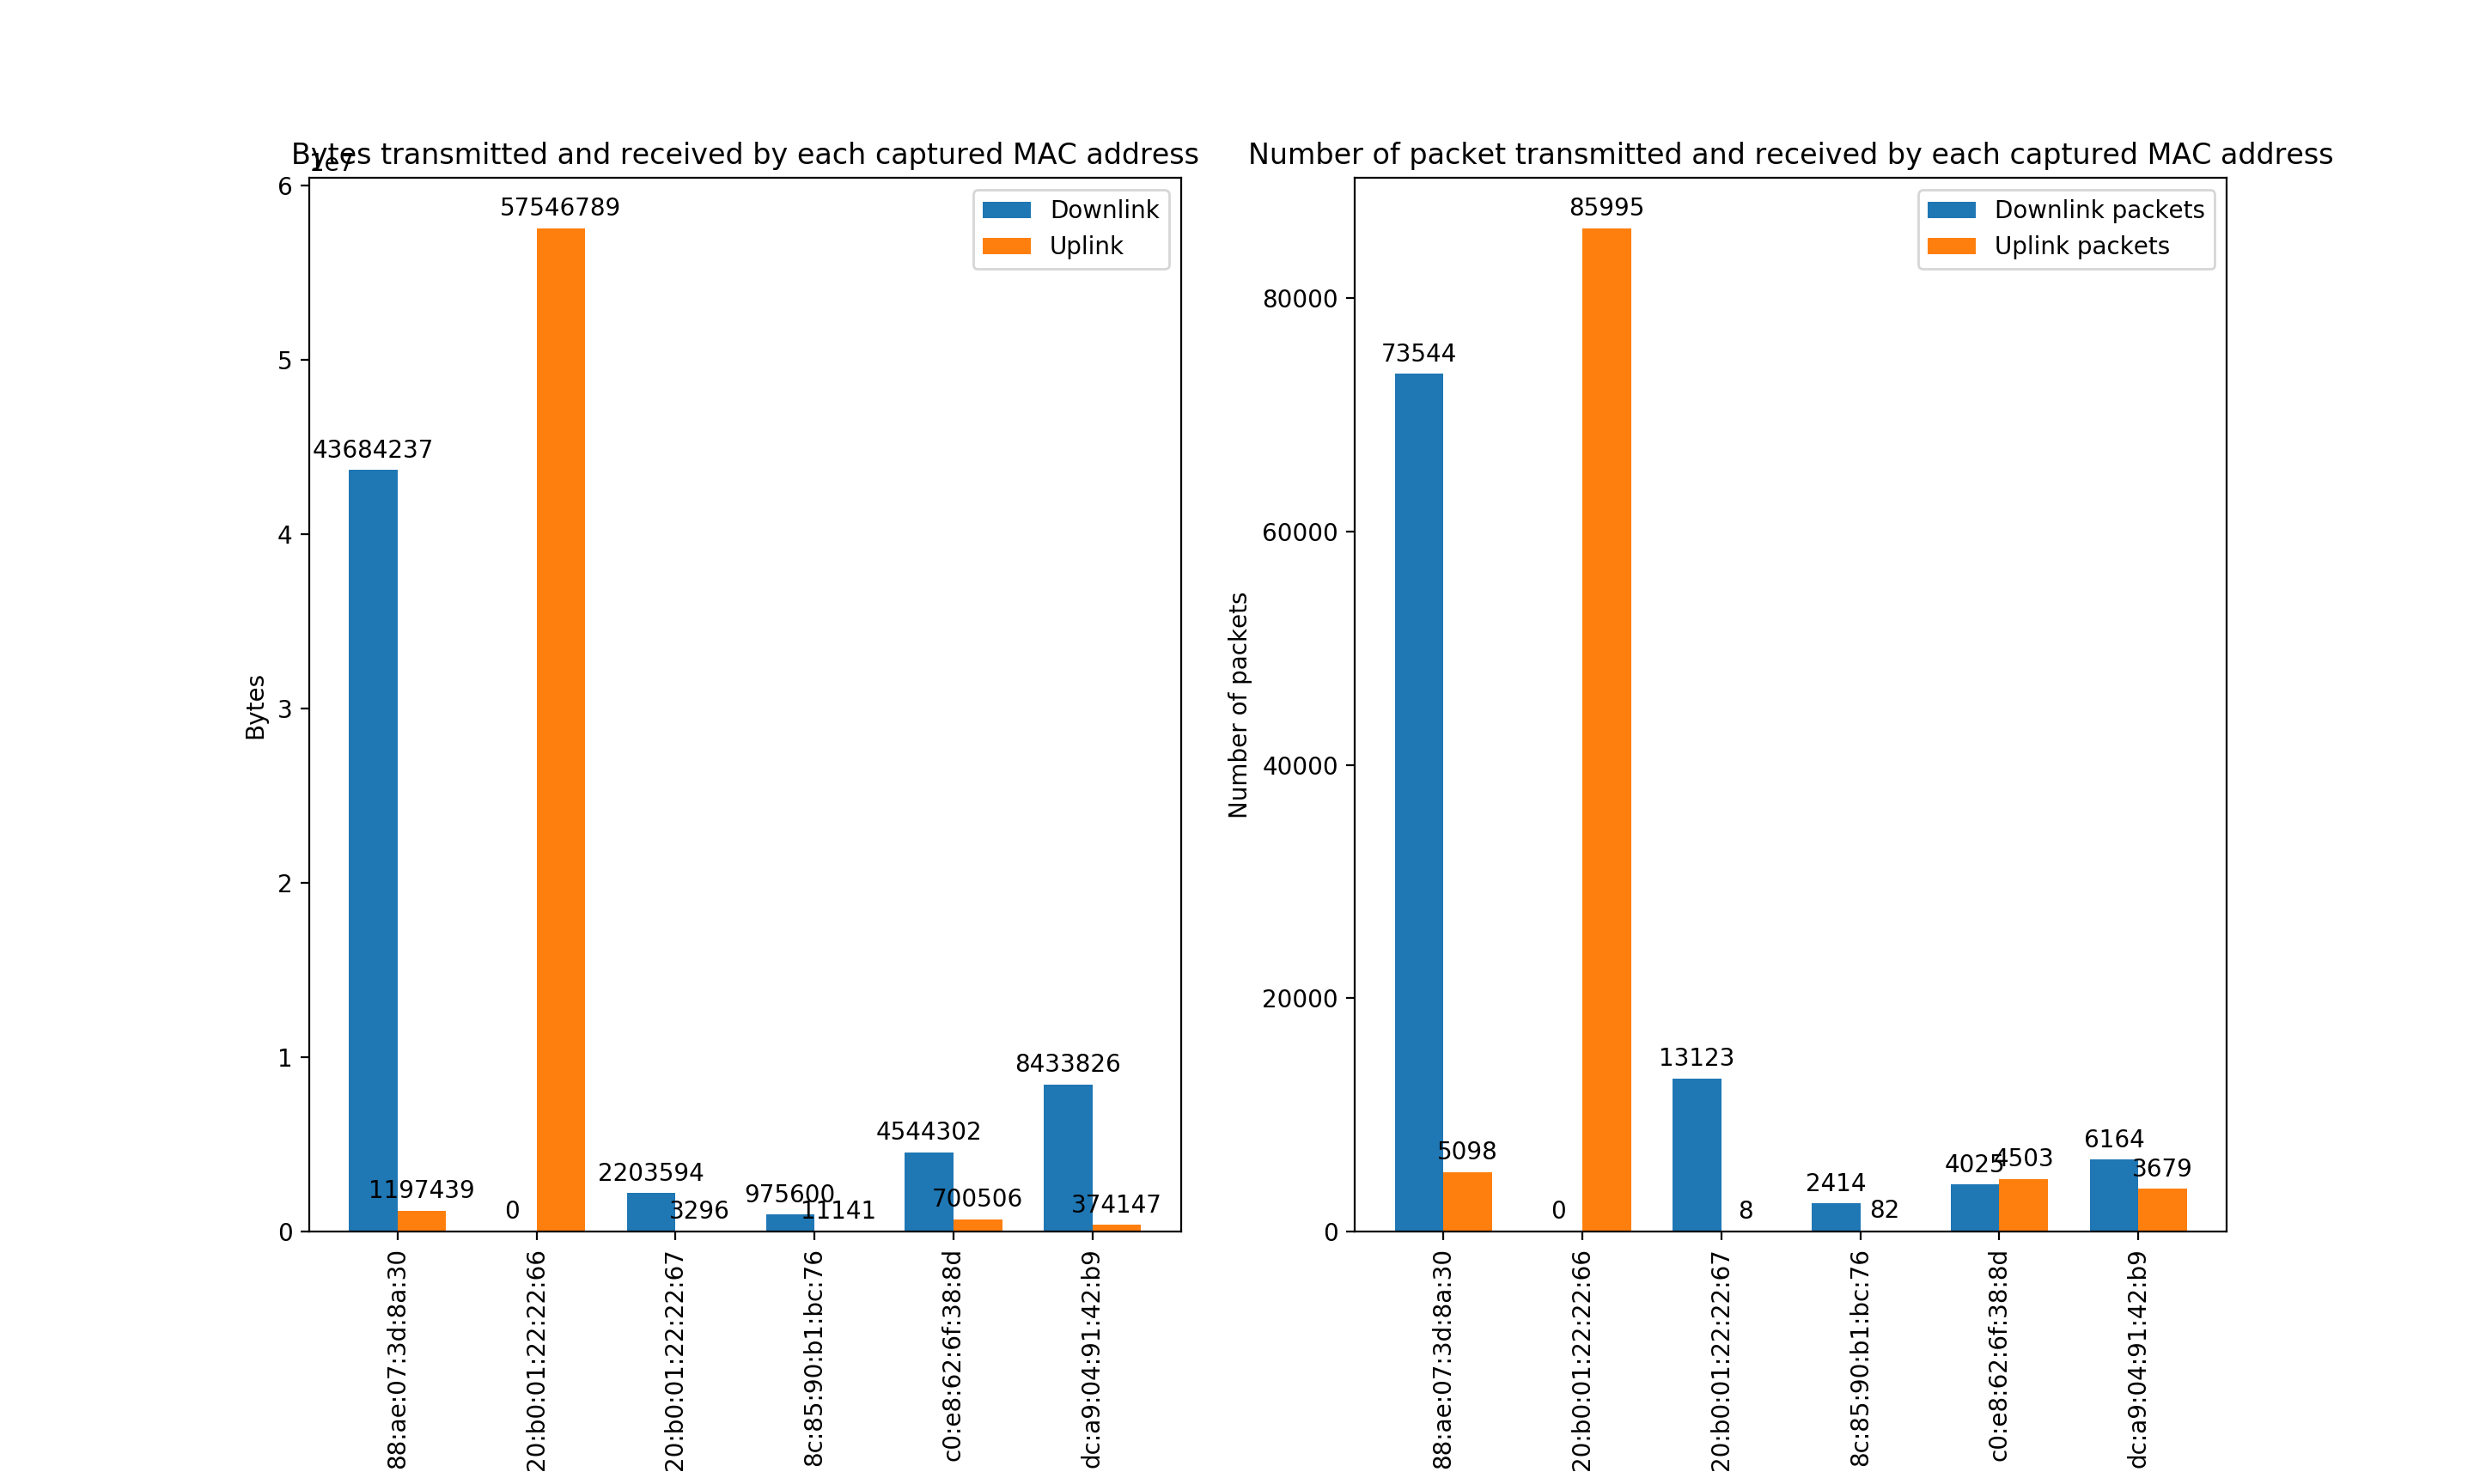
\includegraphics[width=\linewidth]{/Users/lucaferraro/Desktop/PoliMi/First_year/Wireless_networks/Wirelesss_internet/Wireless_internet_project/Graphs/Multimedia_internet_bytes_packets.png}
    \caption{Multimedia internet lecture: data and packets exchanged.}
    \label{fig:Multimedia internet lecture: data and packets exchanged.}
\end{figure}




\subsection{Launch time capture.}
%Luca